%%%%%%%%%%%%%%%%%%%%%%%%%%%%% Define Article %%%%%%%%%%%%%%%%%%%%%%%%%%%%%%%%%%
\documentclass{article}
%%%%%%%%%%%%%%%%%%%%%%%%%%%%%%%%%%%%%%%%%%%%%%%%%%%%%%%%%%%%%%%%%%%%%%%%%%%%%%%

%%%%%%%%%%%%%%%%%%%%%%%%%%%%% Using Packages %%%%%%%%%%%%%%%%%%%%%%%%%%%%%%%%%%
\usepackage{geometry}
\usepackage{graphicx}
\usepackage{amssymb}
\usepackage{amsmath}
\usepackage{amsthm}
\usepackage{empheq}
\usepackage{mdframed}
\usepackage{booktabs}
\usepackage{lipsum}
\usepackage{graphicx}
\usepackage{color}
\usepackage{psfrag}
\usepackage{pgfplots}
\usepackage{bm}
%%%%%%%%%%%%%%%%%%%%%%%%%%%%%%%%%%%%%%%%%%%%%%%%%%%%%%%%%%%%%%%%%%%%%%%%%%%%%%%

% Other Settings

%%%%%%%%%%%%%%%%%%%%%%%%%% Page Setting %%%%%%%%%%%%%%%%%%%%%%%%%%%%%%%%%%%%%%%
\geometry{a4paper}

%%%%%%%%%%%%%%%%%%%%%%%%%% Define some useful colors %%%%%%%%%%%%%%%%%%%%%%%%%%
\definecolor{ocre}{RGB}{243,102,25}
\definecolor{mygray}{RGB}{243,243,244}
\definecolor{deepGreen}{RGB}{26,111,0}
\definecolor{shallowGreen}{RGB}{235,255,255}
\definecolor{deepBlue}{RGB}{61,124,222}
\definecolor{shallowBlue}{RGB}{235,249,255}
%%%%%%%%%%%%%%%%%%%%%%%%%%%%%%%%%%%%%%%%%%%%%%%%%%%%%%%%%%%%%%%%%%%%%%%%%%%%%%%

%%%%%%%%%%%%%%%%%%%%%%%%%% Define an orangebox command %%%%%%%%%%%%%%%%%%%%%%%%
\newcommand\orangebox[1]{\fcolorbox{ocre}{mygray}{\hspace{1em}#1\hspace{1em}}}
%%%%%%%%%%%%%%%%%%%%%%%%%%%%%%%%%%%%%%%%%%%%%%%%%%%%%%%%%%%%%%%%%%%%%%%%%%%%%%%

%%%%%%%%%%%%%%%%%%%%%%%%%%%% English Environments %%%%%%%%%%%%%%%%%%%%%%%%%%%%%
\newtheoremstyle{mytheoremstyle}{3pt}{3pt}{\normalfont}{0cm}{\rmfamily\bfseries}{}{1em}{{\color{black}\thmname{#1}~\thmnumber{#2}}\thmnote{\,--\,#3}}
\newtheoremstyle{myproblemstyle}{3pt}{3pt}{\normalfont}{0cm}{\rmfamily\bfseries}{}{1em}{{\color{black}\thmname{#1}~\thmnumber{#2}}\thmnote{\,--\,#3}}
\theoremstyle{mytheoremstyle}
\newmdtheoremenv[linewidth=1pt,backgroundcolor=shallowGreen,linecolor=deepGreen,leftmargin=0pt,innerleftmargin=20pt,innerrightmargin=20pt,]{theorem}{Theorem}[section]
\theoremstyle{mytheoremstyle}
\newmdtheoremenv[linewidth=1pt,backgroundcolor=shallowBlue,linecolor=deepBlue,leftmargin=0pt,innerleftmargin=20pt,innerrightmargin=20pt,]{definition}{Definition}[section]
\theoremstyle{myproblemstyle}
\newmdtheoremenv[linecolor=black,leftmargin=0pt,innerleftmargin=10pt,innerrightmargin=10pt,]{problem}{Problem}[section]
%%%%%%%%%%%%%%%%%%%%%%%%%%%%%%%%%%%%%%%%%%%%%%%%%%%%%%%%%%%%%%%%%%%%%%%%%%%%%%%

%%%%%%%%%%%%%%%%%%%%%%%%%%%%%%% Plotting Settings %%%%%%%%%%%%%%%%%%%%%%%%%%%%%
\usepgfplotslibrary{colorbrewer}
\pgfplotsset{width=8cm,compat=1.9}
%%%%%%%%%%%%%%%%%%%%%%%%%%%%%%%%%%%%%%%%%%%%%%%%%%%%%%%%%%%%%%%%%%%%%%%%%%%%%%%

%%%%%%%%%%%%%%%%%%%%%%%%%%%%%%% Title & Author %%%%%%%%%%%%%%%%%%%%%%%%%%%%%%%%
\title{Title}
\author{Haoyun Qin}
%%%%%%%%%%%%%%%%%%%%%%%%%%%%%%%%%%%%%%%%%%%%%%%%%%%%%%%%%%%%%%%%%%%%%%%%%%%%%%%

\begin{document}
    \maketitle
    \definecolor{c833431}{HTML}{000000}
    \begin{align*}
    \begin{tikzpicture}
    \begin{axis}[
    	legend pos=outer north east,
    	title=Example,
    	axis lines = middle,
    	xlabel = $x$,
    	ylabel = $y$,
    	domain=-250:250,
    	variable = t,
    	trig format plots = rad,
    ]
    \addplot [
    	samples=70,
    	color=c833431
    ]
    	{126.34453781512605 + 0.7563025210084033 * x ^ 1};
    \addlegendentry{$y=126.3 + 0.756x$}
    \end{axis}
    \end{tikzpicture}
    \end{align*}
    \definecolor{c3670582}{HTML}{000000}
    \begin{align*}
    \begin{tikzpicture}
    \begin{axis}[
    	legend pos=outer north east,
    	title=Example,
    	axis lines = middle,
    	xlabel = $x$,
    	ylabel = $y$,
    	domain=-250:250,
    	variable = t,
    	trig format plots = rad,
    ]
    \addplot [
    	samples=70,
    	color=c3670582
    ]
    	{-453.94677871148366 + 2.0054945054945037 * x ^ 1 + 0.04163973281620334 * x ^ 2};
    \addlegendentry{$y=-453.9 + 2.005x + 0.042x ^ 2$}
    \end{axis}
    \end{tikzpicture}
    \end{align*}
    
    \begin{tikzpicture}
    \begin{axis}[
    legend pos=outer north east,
    title=Example,
    axis lines = box,
    xlabel = $x$,
    ylabel = $y$,
    variable = t,
    trig format plots = rad,
    ]
    \addplot [
        domain=0:5,
        samples=70,
        color=blue,
        ]
        {3*x+4};
    \addlegendentry{$ y=3x+4$}

    \addplot [
        domain=0:2*3.14159265,
        samples=70,
        color=red,
        ]
        ({3*cos(t)+2},{3*sin(t)+4});
    \addlegendentry{$(x-2)^2+(y-4)^2=3^2$}
    \end{axis}
    \end{tikzpicture}
    
    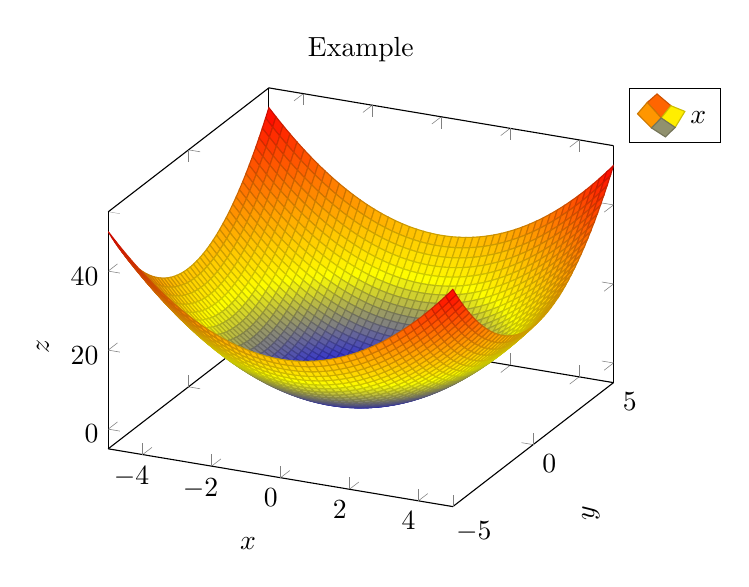
\begin{tikzpicture}
    \begin{axis}[
    legend pos=outer north east,
    title=Example,
    axis lines = box,
    colormap/hot,
    xlabel = $x$,
    ylabel = $y$,
    zlabel = $z$,
    variable = t,
    trig format plots = rad,
    ]
    \addplot3[
        surf,
        samples=50,
    ]
    {x^2+y^2};
    \addlegendentry{$x$}
    \end{axis}
    \end{tikzpicture}

\end{document}